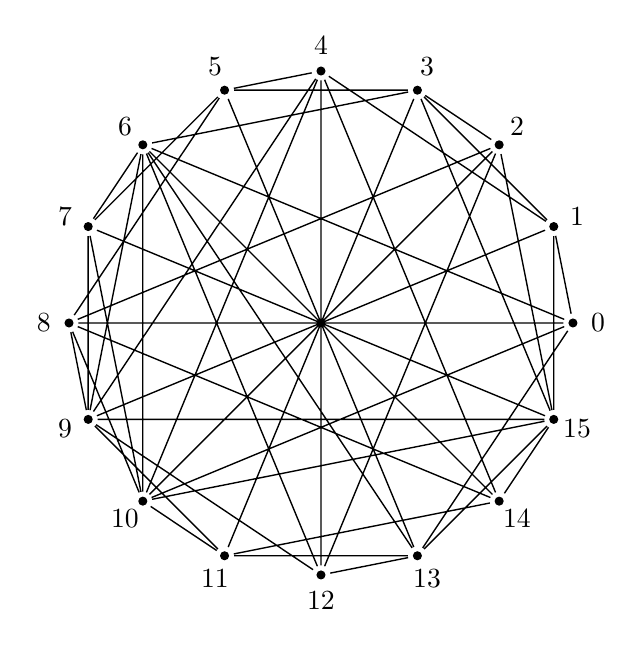
\begin{tikzpicture}[node distance=2cm,scale = .8]
% Vértices
\tikzset{black vertex/.style={circle,draw,minimum size=1mm,inner sep=0pt,outer sep=2pt,fill=black, color=black}}

\foreach \x in {0,...,15}{
    \node[black vertex] (\x) at (\x*360/16:4) {};
	\node () at (\x*360/16:4.4) {\x};
}


% \draw[line width = .5pt] (0) -- (1) (2) -- (3) (4) -- (5) (6) -- (7) (8) -- (9) (10) -- (11) (12) -- (13) (14) -- (15);

\draw[line width = .5pt] (0) -- (1) (0) -- (6) (0) -- (8) (0) -- (10) (0) -- (13) (1) -- (3) (1) -- (4) (1) -- (9) (1) -- (15) (2) -- (3) (2) -- (8) (2) -- (10) (2) -- (12) (2) -- (15) (3) -- (5) (3) -- (6) (3) -- (11) (4) -- (5) (4) -- (10) (4) -- (12) (4) -- (14) (5) -- (7) (5) -- (8) (5) -- (13) (6) -- (7) (6) -- (12) (6) -- (14) (7) -- (9) (7) -- (10) (7) -- (15) (8) -- (9) (8) -- (14) (9) -- (11) (9) -- (12) (10) -- (11) (11) -- (13) (11) -- (14) (12) -- (13) (13) -- (15) (14) -- (15)
(3) -- (15) (4) -- (9) (6) -- (9) (6) -- (10) (6) -- (13) (8) -- (10) (9) -- (15) (10) -- (15);


\end{tikzpicture}